\immediate\write18{tex calligraphy.dtx}
\immediate\write18{tex spath.dtx}
\documentclass{ltxdoc}
\usepackage[T1]{fontenc}
\usepackage{lmodern}
\usepackage{morefloats}
\usepackage{tikz}
\usetikzlibrary{decorations.pathreplacing,matrix}
\usepackage{calligraphy}
\usepackage[numbered]{hypdoc}
\definecolor{lstbgcolor}{rgb}{0.9,0.9,0.9} 
 
\usepackage{listings}
\lstloadlanguages{[LaTeX]TeX}
\lstset{breakatwhitespace=true,breaklines=true,language=TeX}
 
\usepackage{fancyvrb}

\newenvironment{example}
  {\VerbatimEnvironment
   \begin{VerbatimOut}{example.out}}
  {\end{VerbatimOut}
   \begin{center}
   \setlength{\parindent}{0pt}
   \fbox{\begin{minipage}{.9\linewidth}
     \lstset{breakatwhitespace=true,breaklines=true,language=TeX,basicstyle=\small}
     \lstinputlisting[]{example.out}
   \end{minipage}}

   \fbox{\begin{minipage}{.9\linewidth}
     \input{example.out}
   \end{minipage}}
\end{center}
}

\providecommand*{\url}{\texttt}
\GetFileInfo{calligraphy.sty}

\title{The \textsf{calligraphy} Package: Documentation}
\author{Andrew Stacey \\ \url{stacey@math.ntnu.no}}
\date{\fileversion~from \filedate}

\begin{document}

\maketitle
% \section{Introduction}
The \Verb+calligraphy+ package is designed to enable calligraphic style drawings in TikZ.
The idea is to be able to ``stroke'' a line with a ``pen''.
As a simple example, compare the two lines in the following picture.
\begin{example}
\begin{center}
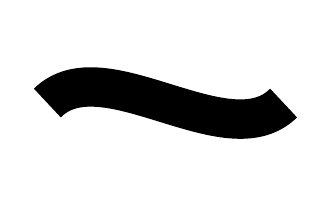
\begin{tikzpicture}
\pen (-135:.25) -- (45:.25);
\draw[line width=.5cm] (0,0) .. controls +(45:1) and +(-135:1) .. ++(3,0);
\calligraphy (0,-1) .. controls +(45:1) and +(-135:1) .. ++(3,0);
\end{tikzpicture}
\end{center}
\end{example}
The paths are identical in definition but the first is drawn using the standard TikZ path with a line width of .5cm.
The second is ``stroked'' with a calligraphic pen of width .5cm angled at 45 degrees.
\section{How It Works}
To know how to use this package, it is worth knowing a little about how it works.
A ``pen'' is a path, as is the line that is the template for the pen stroke.
The two paths are joined together to form a region which is filled.
Thus in constructing the example given in the introduction, the following path is built.
\begin{center}
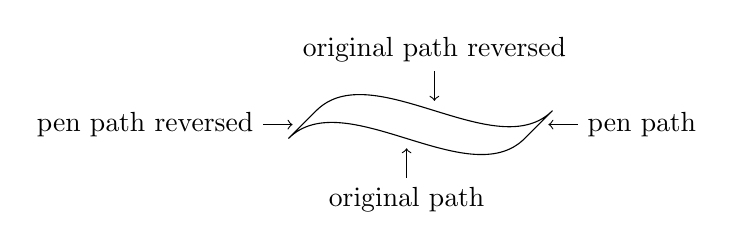
\begin{tikzpicture}
\draw (0,-1) .. controls +(45:1) and +(-135:1) .. node (op) {} ++(3,0) -- node (pp) {} ++(45:.5) .. controls +(-135:1) and +(45:1) .. node (opr) {} ++(-3,0) -- node (ppr) {} (0,-1);
\draw[<-] (op) -- ++(0,-.5) node[anchor=north] {original path};
\draw[<-] (pp) -- ++(.5,0) node[anchor=west] {pen path};
\draw[<-] (opr) -- ++(0,.5) node[anchor=south] {original path reversed};
\draw[<-] (ppr) -- ++(-.5,0) node[anchor=east] {pen path reversed};
\end{tikzpicture}
\end{center}
What is important to note about this is that the ``pen'' isn't \emph{actually} dragged along the path, it is merely a simulation.
This can be shown with the following simple example.
The first is a continuous path that goes past the angle of the pen and thus the upstroke would involve pushing the pen.
The second is how it is meant to be done, the second line is drawn from top to bottom.
However, as the direction of the path isn't important, the same effect can be obtained by ``lifting the nib'' between the lines.
\begin{example}
\begin{center}
\begin{tikzpicture}
\pen (-135:.125) -- (45:.125);
\calligraphy (0,0) -- (1,0) -- (1,1);
\calligraphy (2,0) -- (3,0) (3,1) -- (3,0);
\calligraphy (4,0) -- (5,0) +(0,0) -- (5,1);
\end{tikzpicture}
\end{center}
\end{example}
However, it should work as expected providing the following golden rule is not violated:
\begin{quotation}
Never \emph{push} a calligraphic pen.
\end{quotation}
This is good advice for ordinary calligraphy as well, so a path that is realisable as an honest calligraphic path should be fine with this package.
Actually since, as remarked above, the direction of the path isn't important, a more accurate golden rule would be that one should never swap from pushing to pulling or vice versa without lifting the pen off the paper; but that isn't as succinct.
The paths for both pens and templates can be reasonably complicated.
They can contain gaps, but should not contain closed paths, nor rectangles.
The implementation works by breaking a path into its constituent pieces (broken up by ``move to''s) and working bit by bit.
\begin{example}
\begin{center}
\begin{tikzpicture}
\pen (-135:.25) -- (-135:.125) (45:.125) -- (45:.25);
\calligraphy (0,0) .. controls +(45:1) and +(-135:1) .. +(3,0) ++(1.5,0) .. controls +(-135:2) and +(45:2) .. +(0,-4)  (0,-4) .. controls +(45:1) and +(-135:1) .. +(3,0);
\end{tikzpicture}
\end{center}
\end{example}
\section{Copperplate}
Copperplate pens are somewhat special.
They are ``thin'' so don't need the same treatment as a ``thick'' pen, but one should be able to vary the pressure with a copperplate pen to get a variation of thickness.
Specifying a copperplate pen is straightforward: it is a pen with no thickness.
\begin{example}
\begin{center}
\begin{tikzpicture}[line width=2pt]
\pen (0,0);
\calligraphy[heavy] (0,0) .. controls +(45:1) and +(-135:1) .. +(3,0) ++(1.5,0) .. controls +(-135:2) and +(45:2) .. +(0,-3)  (0,-3) .. controls +(45:1) and +(-135:1) .. +(3,0);
\calligraphy[light] (4,0) .. controls +(45:1) and +(-135:1) .. +(3,0) ++(1.5,0) .. controls +(-135:2) and +(45:2) .. +(0,-3)  (4,-3) .. controls +(45:1) and +(-135:1) .. +(3,0);
\end{tikzpicture}
\end{center}
\end{example}
With a copperplate pen, the segments of a path are tapered.
Copperplate and normal pens can be mixed.
Any part of the pen specification that has no length is treated as a copperplate pen.
\begin{example}
\begin{center}
\begin{tikzpicture}[line width=1pt]
\pen (-135:.125) -- (0,0) (45:.125);
\calligraphy (0,0) .. controls +(45:1) and +(-135:1) .. +(3,0) ++(1.5,0) .. controls +(-135:2) and +(45:2) .. +(0,-3)  (0,-3) .. controls +(45:1) and +(-135:1) .. +(3,0);
\end{tikzpicture}
\end{center}
\end{example}
\section{Annotations}
As an addition, calligraphic paths can be annotated to show how they were constructed.
A path with an arrow is drawn at a set offset from the last part of the path.
\begin{example}
\begin{center}
\begin{tikzpicture}[line width=1pt]
\pen (-135:.125) -- (0,0) (45:.125);
\calligraphy[annotate] (0,0) .. controls +(45:1) and +(-135:1) .. +(3,0) ++(1.5,0) .. controls +(-135:2) and +(45:2) .. +(0,-3)  (0,-3) .. controls +(45:1) and +(-135:1) .. +(3,0);
\end{tikzpicture}
\end{center}
\end{example}
\section{Style Options}
There are plenty of options for styling the paths and pens.
\subsection{Definition Options}
Internally, making a pen is a two-step process.
First a pen has to be \emph{defined} and then \emph{processed}.
To define a pen, the user has to specify a path.
That path is stored in a global macro and so can be accessed in throughout the document.
However, before being used, the pen has to be processed.
At this stage, the pen is converted from a macro in to a special object.
These special objects are local and cannot (at present) be made global.
Thus whilst a pen can be \emph{defined} inside a group, the \emph{processing} stage has to happen in the outermost group in which the pen is going to be used.
There is a shortcut command that (via a bit of suspicious hackery) does all this within a \Verb+tikzpicture+ group.
However, if a pen is to be used in several different pictures, it must be processed outside the group in which it is defined.
The following macros and keys are used to set up and use a pen.
All the keys are in the \Verb+/pgf/calligraphy+ family.
\begin{itemize}
\item \DescribeMacro{define pen}If the \Verb+define pen+ key is specified on a path then that path will be used to define a pen.
It can take one option which will be the pen name, if not specified then \Verb+default+ is assumed.
The resulting path will not be counted for bounding box considerations.
When the pen is used, the origin will correspond to the path along which it is dragged.
\item \DescribeMacro{pen name}The key \Verb+pen name=name+ sets the name for the current pen.
This can be used either when defining or using a pen.
\item \DescribeMacro{\pen}\DescribeMacro{\definepen}The macros \Verb+\pen+ and \Verb+\definepen+ are analogous to the TikZ commands \Verb+\draw+ or \Verb+\fill+ in that it acts like a path command but stores the path as a pen.
(The two macros are the same.)
These macros also change the ``key family'' to \Verb+/pgf/calligraphy+ so that any further options do not need their full path.
\item \DescribeMacro{\processpen}The macro \Verb+\processpen+ processes a pen so that it is set up for using later on.
As remarked earlier, it has to be given at least at the outermost grouping of where it will be used.
It takes an optional argument which is the pen name.
This is only needed if the pen will be used in a group other than the one in which it is defined (or if the hackery that means this isn't needed with the \Verb+\pen+ command fails for some unknown reason).
\item \DescribeMacro{use pen}The key \Verb+use pen=name+ on a path means that that path should be ``stroked'' with the pen (\Verb+default+ if no name is given, or none specified via the \Verb+pen name+ key).
\item \DescribeMacro{\calligraphy}The macro \Verb+\calligraphy+ is a shortcut for specifying a path with the key \Verb+use pen+ already set.
This macro also changes the ``key family'' to \Verb+/pgf/calligraphy+ so that any further options do not need their full path.
\end{itemize}
\subsection{Style Options}
There are various options available for styling the calligraphic paths.
All of these are in the \Verb+/pgf/calligraphy+ key family, but the \Verb+\calligraphy+ command automatically switches to that family so the key path is not needed.
Any unknown keys are processed as follows:
\begin{enumerate}
\item A check is made to see if a pen of that name has been defined.
If so, that pen is used.
This is similar to the \Verb+\node[shape]+ syntax
\item A check is made to see if the unknown key corresponds to a colour.
If so, that colour is installed as the pen colour.
This is similar to the colour handling of TikZ paths.
(In fact, it uses the same code.)
\item All other unknown options are passed on to TikZ.
\end{enumerate}
The style options are as follows.
\begin{itemize}
\item \DescribeMacro{pen colour}The \Verb+pen colour+ style defines the default colour to be used.
Since calligraphic paths are sometimes filled and sometimes stroked, this ensures that the colour is used correctly.
\item \DescribeMacro{pen nib}It is possible to style particular ``nibs'' (i.e., segments of the pen path) separately.
This is the \Verb+pen nib+ option, which takes two arguments.
The first is the index of the part of the nib and the second is the style options to be applied.
\item \DescribeMacro{line style}It is also possible to style particular parts of the template path.
This is done by putting \Verb+[line style={}]+ in the template path at the relevant part.
The style is saved and applied to that segment of the template path.
\item \DescribeMacro{taper}The tapering of copperplate paths can be controled by the \Verb+taper+ option.
It takes arguments \Verb+none+, \Verb+both+, \Verb+start+, and \Verb+end+.
\item \DescribeMacro{weight}\DescribeMacro{heavy}\DescribeMacro{light}Copperplate paths come in two ``weights'': \emph{heavy} and \emph{light}.
The weight also affects the tapering: by default a light path is tapered to nothing whilst a heavy path is tapered to the width of a light path.
Weights can be specified by either \Verb+weight=weight+ or just \Verb+heavy+ and \Verb+light+.
It is possible to change the weight for different components of a path using the \Verb+line style+ key.
With tapering, this means that one can easily vary from a light stroke to a heavy one.
The relevant widths are controlled by the keys \DescribeMacro{heavy line width}\Verb+heavy line width+ and the \DescribeMacro{light line width}\Verb+light line width+.
The \DescribeMacro{taper line width}\Verb+taper line width+, is set automatically by the weight but can be altered afterwards using the \Verb+taper line width+ key.
\item \DescribeMacro{annotate}The key \Verb+annotate+ switches on annotations.
The style of the annotations is controlled by the keys \DescribeMacro{annotation style}\Verb+annotation style+, \DescribeMacro{annotation shift}\Verb+annotation shift+ which controls how the annotation path is shifted from the final component of the calligraphic path, \DescribeMacro{annotation nodes style}\Verb+annotation nodes style+ for global style of the nodes, \DescribeMacro{annotation node style}\Verb+annotation node style+ for styling of particular nodes.
This latter takes two options: the node number and the style to be applied.
The annotation path and annotation node styles take ordinary TikZ styling options.
\end{itemize}
\begin{example}
\begin{center}
\processpen
\begin{tikzpicture}
\calligraphy[pen colour=green,pen nib={2}{color=red}] (0,0) .. controls +(45:1) and +(-135:1) .. +(3,0) ++(1.5,0) .. controls +(-135:2) and +(45:2) .. +(0,-3)  (0,-3) .. controls +(45:1) and +(-135:1) .. +(3,0);
\calligraphy[annotate,annotation node style={2}{circle,draw,fill=white}] (4,0) .. controls +(45:1) and +(-135:1) .. +(3,0) ++(1.5,0) .. controls +(-135:2) and +(45:2) .. +(0,-3)  (4,-3) .. controls +(45:1) and +(-135:1) .. +(3,0);
\calligraphy[pen nib style={line width=1pt}] (0,-4) .. controls +(45:1) and +(-135:1) .. +(3,0) ++(1.5,0) .. controls +(-135:2) and +(45:2) .. +(0,-3)  (0,-7) .. controls +(45:1) and +(-135:1) .. +(3,0);
\calligraphy[annotate,annotation style={dashed,->}] (4,-4) .. controls +(45:1) and +(-135:1) .. +(3,0) ++(1.5,0) .. controls +(-135:2) and +(45:2) .. +(0,-3)  (4,-7) .. controls +(45:1) and +(-135:1) .. +(3,0);
\end{tikzpicture}
\end{center}
\end{example}
\section{Decorations}
If a TikZ/PGF decorations library is loaded prior to this package, then the \Verb+calligraphy+ package defines some decorations that use the calligraphic paths, specifically with the copperplate nib.
The current decorations are:
\begin{itemize}
\item \DescribeMacro{calligraphic brace}\Verb+calligraphic brace+ for a brace.
\item \DescribeMacro{calligraphic straight parenthesis}\Verb+calligraphic straight parenthesis+ for a parenthesis with straight middle component.
\item \DescribeMacro{calligraphic curved parenthesis}\Verb+calligraphic curved parenthesis+ for a parenthesis with a curved middle component.
\end{itemize}
All the above use the \Verb+amplitude+ option to specify their size.
The following is an example of their use, together with the standard \Verb+brace+ and the \Verb+delimiter+ key from the \Verb+matrix+ library for comparison.
\begin{example}
\begin{center}
\begin{tikzpicture}
\draw[decorate,decoration={calligraphic brace,amplitude=4mm},ultra thick] (0,0) -- (0,8);
\draw[line width=2pt,decorate,decoration={brace,amplitude=10},line cap=round] (1,0) -- ++(0,8);
\node[anchor=south west,minimum height=8cm,outer sep=0pt,left delimiter=\{] (a) at (2,0) {};
\draw[decorate,decoration={calligraphic straight parenthesis,amplitude=4mm},ultra thick] (3,0) -- ++(0,8);
\draw[decorate,decoration={calligraphic curved parenthesis,amplitude=4mm},ultra thick] (4,0) -- ++(0,8);
\node[anchor=south west,minimum height=8cm,outer sep=0pt,left delimiter=(] (a) at (5,0) {};
\end{tikzpicture}
\end{center}
\end{example}
\section{Pre-Defined Pens}
The following pens are predefined:
\begin{itemize}
\item \DescribeMacro{copperplate}\Verb+copperplate+:
\begin{example}
\begin{center}
\tikz \calligraphy[copperplate] (0,0) .. controls +(1,-1) and +(-1,1) .. ++(3,0) [calligraphy,line style={light,taper=start}] +(0,0) .. controls +(1,-1) and +(-1,1) .. ++(3,0) [calligraphy,line style={heavy}];
\end{center}
\end{example}
\end{itemize}

\end{document}